\documentclass[xcolor=dvipsnames]{beamer}

\usetheme{Boadilla}

\newcommand{\bi}{\begin{itemize}}
\newcommand{\ei}{\end{itemize}}
\newcommand{\be}{\begin{enumerate}}
\newcommand{\ee}{\end{enumerate}}
\newcommand{\bc}{\begin{center}}
\newcommand{\ec}{\end{center}}
\newcommand{\I}{\item}
\newcommand{\f}{\frame}
\newcommand{\ft}{\frametitle}
\newcommand{\bcol}{\begin{column}}
\newcommand{\ecol}{\end{column}}
\newcommand{\bcols}{\begin{columns}}
\newcommand{\ecols}{\end{columns}}

\title{Two-Pass Track Fitting Method}
\author[M.\ Ito]{Mark M.\ Ito}
\date{October 1, 2008}
\institute[JLab]{Jefferson Lab}

\begin{document}

\frame{\titlepage}

\f{
\ft{Least-Squares Fitter}
\bi
\I Uses Levenberg-Marquardt algorithm from GNU Scientific Library
\I Works with FDC hits, CDC hits, or any combination
\I Current status: Unweighted fit (assume equal measurement errors)
\I Track parameters:
\bi
\I Total inverse momentum: $1/p$
\I Polar angle: $\theta$
\I Azimuthal angle: $\phi$
\I Transverse distance of point of closest approach to beamline: $x^\prime_0$
\I Z of point of closest approach to beamline: $z_0$
\ei
\ei
}

\f{
\ft{Problem: local minima}
\bi
\I rough starting position:
\bi
\I $1/p = 0$
\I $z_0 = 0$
\I $\phi$ and $x^\prime_0$ set by line going through first and last cdc wires
\I theta set to be 45, 90, or 135 degrees whichever is closest to the true $\theta$
\ei
\I Many fits with poor chi-squared (few tens of \%)
\ei
}

\f{
\ft{New approach: flat in the middle}
\bc
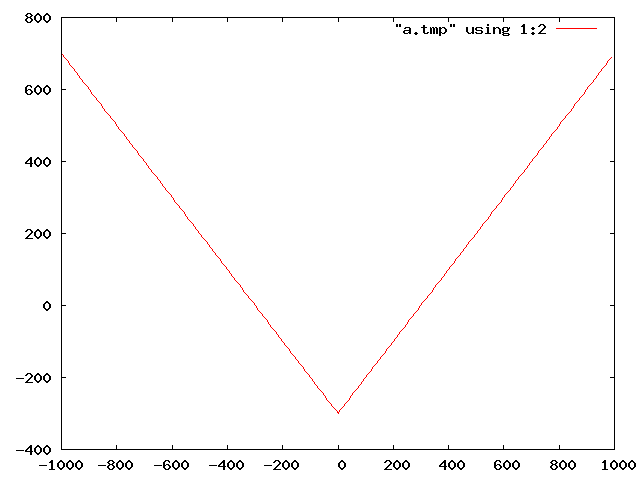
\includegraphics[width=3.0in]{resid1.png}
\ec
Residual vs. position for a 1 mm radius cell and a drift distance of 300 microns.
}

\f{
\bc
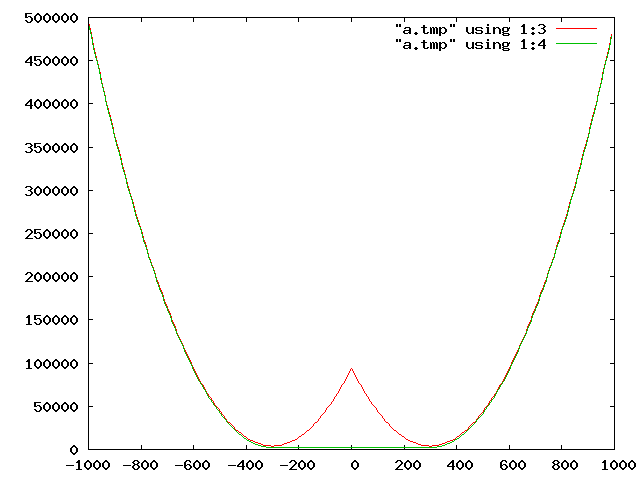
\includegraphics[width=3.0in]{resid2.png}
\ec
Squared residuals for 300 micron drift distance, red: nominal, green: flattened
}

\f{
\bc
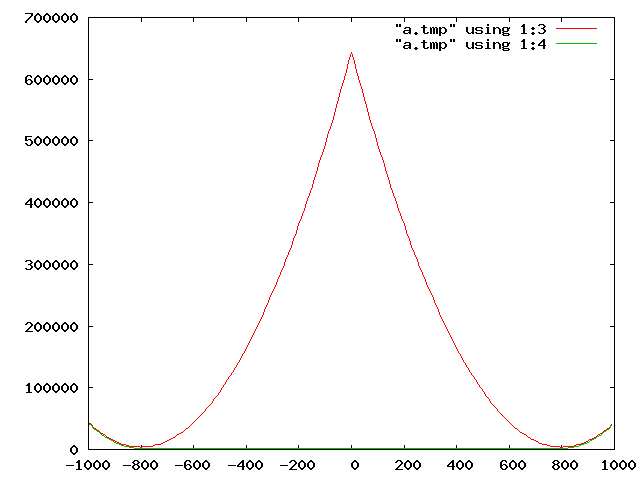
\includegraphics[width=3.0in]{resid2_large.png}
\ec
Squared residuals for 800 micron drift.
}

\f{
\ft{Two-Pass Approach}
\be
\I Fit with modified, flattened residual function
\I Use results as starting point for second fit with standard residual function
\ee
}

\f{
\bc
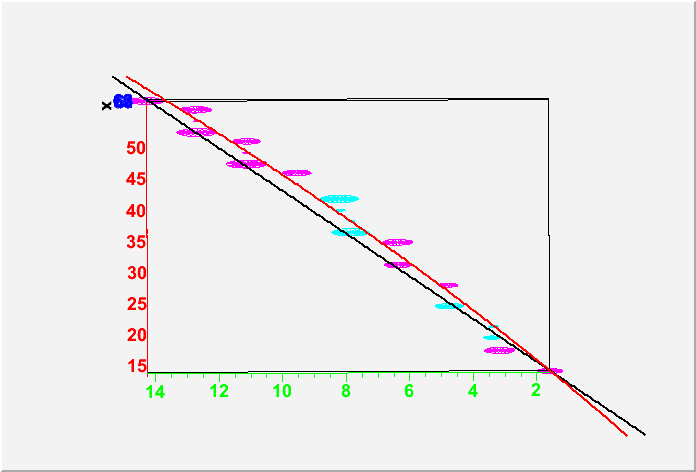
\includegraphics[width=4.0in]{e3_one.png}
\ec
Event 3, one-pass method, chi-squared = 0.600
}

\f{
\bc
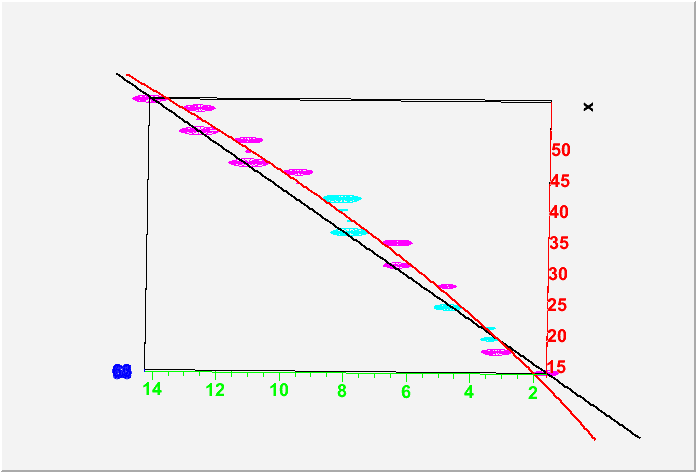
\includegraphics[width=4.0in]{e3_two.png}
\ec
Event 3, two-pass method, chi-squared = 0.030
}

\f{
\ft{Monte Carlo Data Sample}
\bi
\I Positive pions
\I $p = 2.0$~GeV/$c$
\I Uniform in theta and phi
\I Fixed starting point:
\bi
\I $x^\prime_0 = 0$
\I $z0 = 65$~cm
\ei
\I 100,000 events generated
\ei
}

\f{
\bc
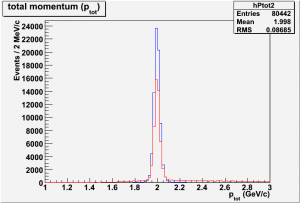
\includegraphics[width=4.0in]{two_pass_p_lin.png}
\ec
Total momentum, one-pass and two-pass methods, linear scale
}

\f{
\bc
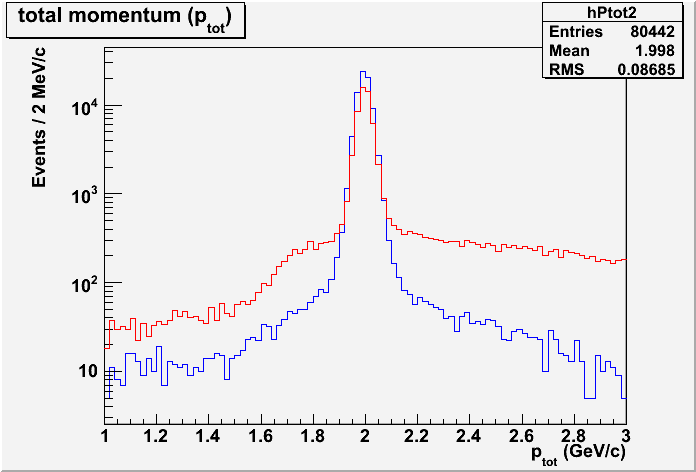
\includegraphics[width=4.0in]{two_pass_p_log.png}
\ec
Total momentum, one-pass and two-pass methods, log scale
}

\f{
\bc
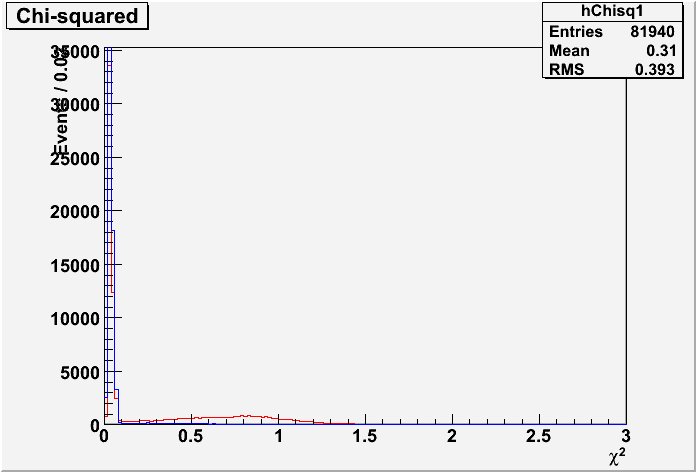
\includegraphics[width=4.0in]{two_pass_chisq_lin.png}
\ec
Chi-squared, one-pass and two-pass methods, linear scale
}

\f{
\bc
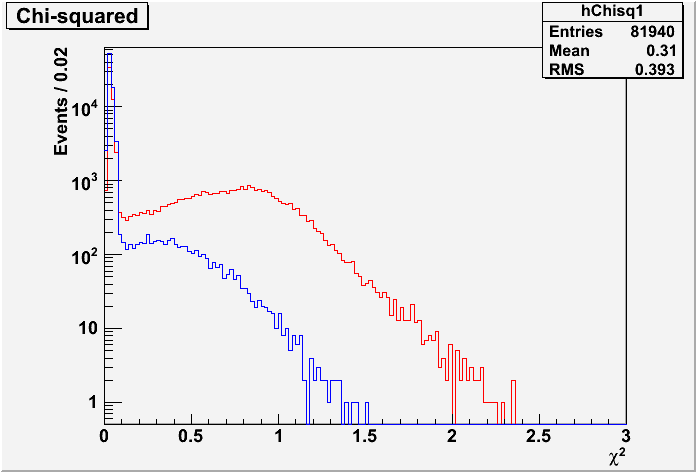
\includegraphics[width=4.0in]{two_pass_chisq_log.png}
\ec
Chi-squared, one-pass and two-pass methods, log scale
}

\f{
\ft{Things to do}
\bi
  \I get the covariance matrix
  \I put in position smearing
  \I try without multiple scattering, energy loss
  \I look at events that still have bad chi-squared
  \I look at residual distributions and scale terms in chi-squared appropriately
  \I try fitting using transverse momentum rather than total momentum
  \I fix events that have bad minimum brackets
\ei
}

\end{document}
